% !TEX root = ../main.tex

\section{Эквивалентный ветер и его связь с реальным ветром}
\textbf{Эквивалентный ветер} – условный ветер, который по направлению совпадает с направлением маршрута; и при данной V он создает такую же W как и реальный ветер.\\
позволяет определить фактическую W при известной V и требуемую V для полета по расписанию c заданной W.

\begin{wrapfigure}[3]{R}{0.56\linewidth}
	\vspace{-6mm}
	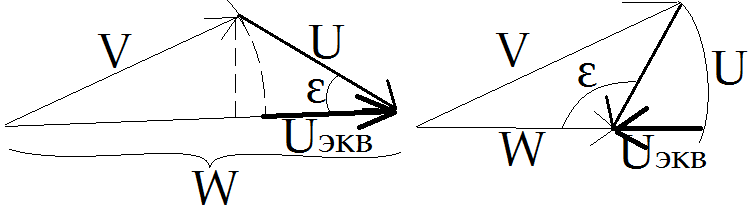
\includegraphics[width=29 mm]{EquivalentWind}
\end{wrapfigure}

$U_\text{экв}=W-V$\\
$\varepsilon=\delta_\text{н}-\text{МПУ}$\\
$\alpha$ - путевой угол\\
 $U_\text{эк}$=$U_\text{прод}$-$\frac{U_\text{бок}^2}{2V}$; $U_\text{эк}$=$Vcos\varepsilon$-$\frac{U^2}{2V}sin^2\varepsilon$
